
%%%%%%%%%%%%%%%%%%%%%%% file typeinst.tex %%%%%%%%%%%%%%%%%%%%%%%%%
%
% This is the LaTeX source for the instructions to authors using
% the LaTeX document class 'llncs.cls' for contributions to
% the Lecture Notes in Computer Sciences series.
% http://www.springer.com/lncs       Springer Heidelberg 2006/05/04
%
% It may be used as a template for your own input - copy it
% to a new file with a new name and use it as the basis
% for your article.
%
% NB: the document class 'llncs' has its own and detailed documentation, see
% ftp://ftp.springer.de/data/pubftp/pub/tex/latex/llncs/latex2e/llncsdoc.pdf
%
%%%%%%%%%%%%%%%%%%%%%%%%%%%%%%%%%%%%%%%%%%%%%%%%%%%%%%%%%%%%%%%%%%%

\iffalse
\documentclass[runningheads,a4paper]{llncs}

\usepackage{amssymb}
\setcounter{tocdepth}{3}
\usepackage{graphicx}

\usepackage{url}
\usepackage{color}

\urldef{\mailsa}\path|{alfred.hofmann, ursula.barth, ingrid.haas, frank.holzwarth,|
\urldef{\mailsb}\path|anna.kramer, leonie.kunz, christine.reiss, nicole.sator,|
\urldef{\mailsc}\path|erika.siebert-cole, peter.strasser, lncs}@springer.com|    
\newcommand{\keywords}[1]{\par\addvspace\baselineskip
\noindent\keywordname\enspace\ignorespaces#1}

\newcommand{\acom[1]}{\textcolor{red}{#1}}


\begin{document}

\mainmatter  % start of an individual contribution

% first the title is needed


% a short form should be given in case it is too long for the running head
\titlerunning{Object Detections' Semantics for Scene Categorization}

% the name(s) of the author(s) follow(s) next
%
% NB: Chinese authors should write their first names(s) in front of
% their surnames. This ensures that the names appear correctly in
% the running heads and the author index.
%

\author{   
% Gregoire Salah Antoine Xavier Yoshua Pascal
Gr\'{e}goire Mesnil$^{1,2}$ \and Salah Rifai$^{1}$
\and Antoine Bordes$^{3}$ \and Xavier Glorot$^{1}$\and\\
Yoshua Bengio$^{1}$ \and Pascal Vincent$^{1}$
}
%\affiliation{\sup{1}LISA, Universit\'{e} de Montr\'{e}al, Qu\'{e}bec, Canada}
%\affiliation{\sup{2}LITIS, Universit\'{e} de Rouen, France}
%\affiliation{\sup{3}CNRS - Heudiasyc UMR 7253, Universit\'{e} de Technologie de Compi\`{e}gne, France}
%\email{gregoire.mesnil@umontreal.ca}
%}


%\author{Alfred Hofmann%
%\thanks{Please note that the LNCS Editorial assumes that all authors have used
%the western naming convention, with given names preceding surnames. This determines
%the structure of the names in the running heads and the author index.}%
%\and Ursula Barth\and Ingrid Haas\and Frank Holzwarth\and\\
%Anna Kramer\and Leonie Kunz\and Christine Rei\ss\and\\
%Nicole Sator\and Erika Siebert-Cole\and Peter Stra\ss er}
%
\authorrunning{Gr\'egoire Mesnil et al.}
% (feature abused for this document to repeat the title also on left hand pages)

% the affiliations are given next; don't give your e-mail address
% unless you accept that it will be published
\institute{
%Springer-Verlag, Computer Science Editorial,\\
%Tiergartenstr. 17, 69121 Heidelberg, Germany\\
%\mailsa\\
%\mailsb\\
%\mailsc\\
%\url{http://www.springer.com/lncs}}
$^{1}$ LISA, Universit\'{e} de Montr\'{e}al, Qu\'{e}bec, Canada\\
$^{2}$ LITIS, Universit\'{e} de Rouen, France\\
$^{3}$ CNRS - Heudiasyc UMR 7253, Universit\'{e} de Technologie de Compi\`{e}gne, France
%
}
%
% NB: a more complex sample for affiliations and the mapping to the
% corresponding authors can be found in the file "llncs.dem"
% (search for the string "\mainmatter" where a contribution starts).
% "llncs.dem" accompanies the document class "llncs.cls".
%

%\toctitle{Lecture Notes in Computer Science}
%\tocauthor{Authors' Instructions}
\maketitle


\begin{abstract} Classifying scenes (e.g. into ``street'', ``home'' or
``leisure'') is an important but complicated task nowadays, because images come
with variability, ambiguity, and a wide range of illumination or scale
conditions.
  %
  Standard approaches build an intermediate representation of the global image
  and learn classifiers on it. %~\citep{Lazebnik06,Lowe99,Csurka04}.
  %
  Recently, it has been proposed to depict an image as an aggregation of its
  contained objects:~ the representation on which classifiers are trained is
  composed of many heterogeneous feature vectors derived from various object
  detectors.
  %
  In this paper, we propose to study different approaches to efficiently learn
  contextual semantics out of these object detections.
  %
  We use the features provided by Object-Bank~\citep{LiJiaLi10} (177 different
  object detectors producing 252 attributes each), and show on several
  benchmarks for scene categorization that careful combinations, taking into
  account the structure of the data, allows to greatly improve over original
  results (from $+5\%$ to $+11\%$)
  %of the original paper (+11\% on MIT Indoor, +5\% on UIUC Sports and +4\% on
  %15-scenes) 
  while drastically reducing the dimensionality of the % Object-Bank
      representation by 97\% (from $44,604$ to $1,000$).
  %
  We also show that the uncertainty relative to object detectors hampers the
  use of external semantic knowledge to improve detectors combination, unlike
  our unsupervised learning approach.

\keywords{Unsupervised Learning, Transfer Learning, Deep Learning, Scene Categorization, Object Detection}
\end{abstract}
\fi

\chapter{Unsupervised Learning of Semantics of Object Detections for Scene Categorization\label{chap:ob}}
\section{Introduction}


Automatic scene categorization is crucial for many applications such
as content-based image indexing \citep{Smeulders:2000} or image
understanding.
%
This is defined as the task of assigning images to predefined
categories ( ``office'', ``sailing'', ``mountain'', etc.).
%
Classifying scene is complicated because of the large variability of
quality, subject and conditions of natural images which lead to many
ambiguities w.r.t. the corresponding scene label.

Standard methods build an intermediate representation before
classifying scenes by considering the image as a whole
\citep{Torralba03,Vogel:2004,FeiFei:2005,Oliva06}. In particular, many
such approaches rely on power spectral information, such as
magnitude of spatial frequencies \citep{Oliva06} or local texture
descriptors \citep{FeiFei:2005}.
%
They have shown to perform well in cases where there are large
numbers of scene categories.

Another line of work conveys promising potential in scene categorization.
%
First applied to object recognition~\citep{Farhadi:2009}, attribute-based
methods have now proved to be effective for dealing with complex scenes.
%
These models define high-level representations by combining semantic
lower-level elements, e.g., detection of object parts.
%
A precursor of this tendency for scenes was an adaptation of
pLSA~\citep{Hofmann:2001} to deal with ``visual words'' proposed by
\citep{Bosh:2006}. 
%
An extension of this idea consists in modeling an image based on its content
i.e. its objects \citep{Espinace10ICRA,LiJiaLi10}. Hence, the Object-Bank (OB)
project~\citep{LiSuLimFeiFei} aims at building high-dimensional over-complete
representations of scenes (of dimension $44,604$) by combining the outputs of
many object detectors ($177$) taken at various poses, scales and positions in
the original image (leading to $252$ attributes per detector).
% I added poses which correspond to root filters G To unify language pose or
% root = pose detector or object = object
%
Experimental results indicate that this approach is effective since simple
classifiers such as Support Vector Machines trained on their representations
achieve state-of-the-art performance.
%
However, this approach suffers from two flaws: (1) curse of dimensionality
(very large number of features) and (2) individual object detectors have a poor
precision (30\% at most).
%
%Solving (2) is beyond the scope of this work.
%
To solve (1), the original paper proposes to use structured norms and group
sparsity to make best use of the large input.
%
%Such good results are simply obtained by learning the classifier on the plain
%concatenation of the attributes extracted by each object detector.
%
Our work studies new ways to combine the very rich information provided by
these multiple detectors, dealing with the uncertainty of the detections.
%
A method designed to select and combine the most informative attributes would
be able to carefully manage redundancy, noise and structure in the data,
leading to better scene categorization performance.


%% NEW STUFF

Hence, in the following, we propose 
%two kinds of strategies 
a sequential $2$-steps strategy for combining the feature representations
provided by the OB object detectors on which the linear SVM classifier is
destined to be trained for categorizing scenes.
%
The first step adapts Principal Components Analysis (PCA) to this particular
setting: we show that it is crucial to take into account the structure of the
data in order for PCA to perform well.
%
The second one is based on {\em Deep Learning}.
%
Deep Learning has emerged recently (see \citep{Bengio-2009} for a review) and is
based on neural network algorithms able to discover data representations in an
unsupervised
fashion~\citep{Hinton06,Bengio-nips-2006-short,ranzato-07-small,Koray-08,Jarrett-ICCV2009}.
%
We propose to use this ability to combine multiple detector features. Hence, we
present 
%several models trained in a parallel fashion 
a model trained using Contractive Auto-Encoders
\citep{Rifai+al-2011,Salah+al-2011}, which have already proved to be efficient
on many image tasks and has contributed to winning a transfer learning
challenge~\citep{UTLC+LISA-2011}.
% Plutot dans le cas general que sur des images tasks non ? on s'attaque a des
% features sans connaissance apriori comme on pourrait l'avoir pour des images
% Gregoire
%
% Antoine: peut-être mais ici il faut justifier pourquoi on utilise des CAE et
% pas des RBM ou des DAE -- une raison peut être leur efficacité sur des images
%
%Object-Bank detector outputs (of dimension $252$) and transforms it
%non-linearly into a smaller vector (of dimension $100$). The second layer
%combines these $177$ compressed feature vectors into a unified representation
%(of dimension $1000$?). 
%% CAE

%Exp
We validate the quality of our models in an extensive set of experiments in
which several setups of the sequential feature extraction process are evaluated
on benchmarks for scene classification
\citep{Lazebnik06,LiJiaLi07,Quattoni09,Xiao:2010}. 
%
 We show that our best results substantially outperform the original methods
 developed on top of OB features, while producing representations of much lower
 dimension.
  %
  The performance gap is usually large, indicating that advanced combinations
  are highly beneficial. 
  % 
  We show that our method based on dimensionality reduction followed by deep
  learning offers a flexibility which makes it able to benefit from
  % transductive,
  semi-supervised and transfer learning.
  %
  %We find that the use of supervised fine-tuning outperforms any of the
  %PCA-based strategies tested.
  %
  %The results on different setups are either state-of-the-art (compared with
  %methods using large combinations of features like \citep{Gao10}) or very
  %close to it. 



%
%We conclude with a discussion of the advantages and drawbacks of both
%combination approaches.

%Antoine: to remove if one needs some space
% The paper is organized as follows. Section~\ref{sec:ob} details
% Object-Bank. Section~\ref{sec:feat} describes the building blocks of
% our combination strategies presented in Section~\ref{sec:combi}. Our
% experimental results are in Section~\ref{sec:exp} and the paper ends
% with a conclusion and discussion of future work in Section~\ref{sec:disc}.

\begin{figure*}
\begin{center}
\begin{tabular}{ccc}
  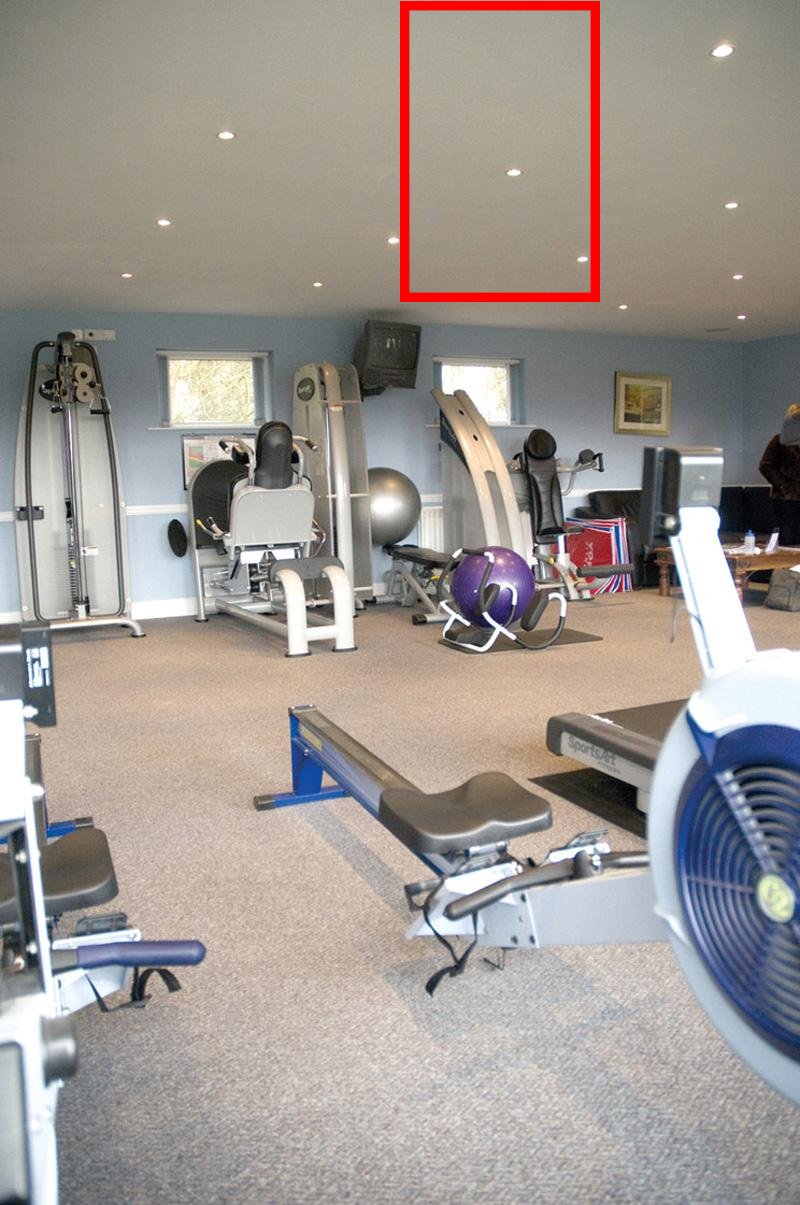
\includegraphics[height=0.20\linewidth]{article2/images/cloud1.png}&
  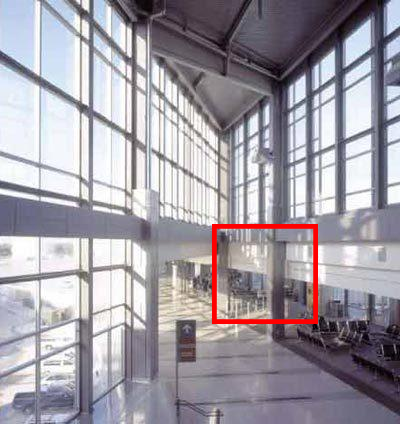
\includegraphics[height=0.20\linewidth]{article2/images/man1.png} &
  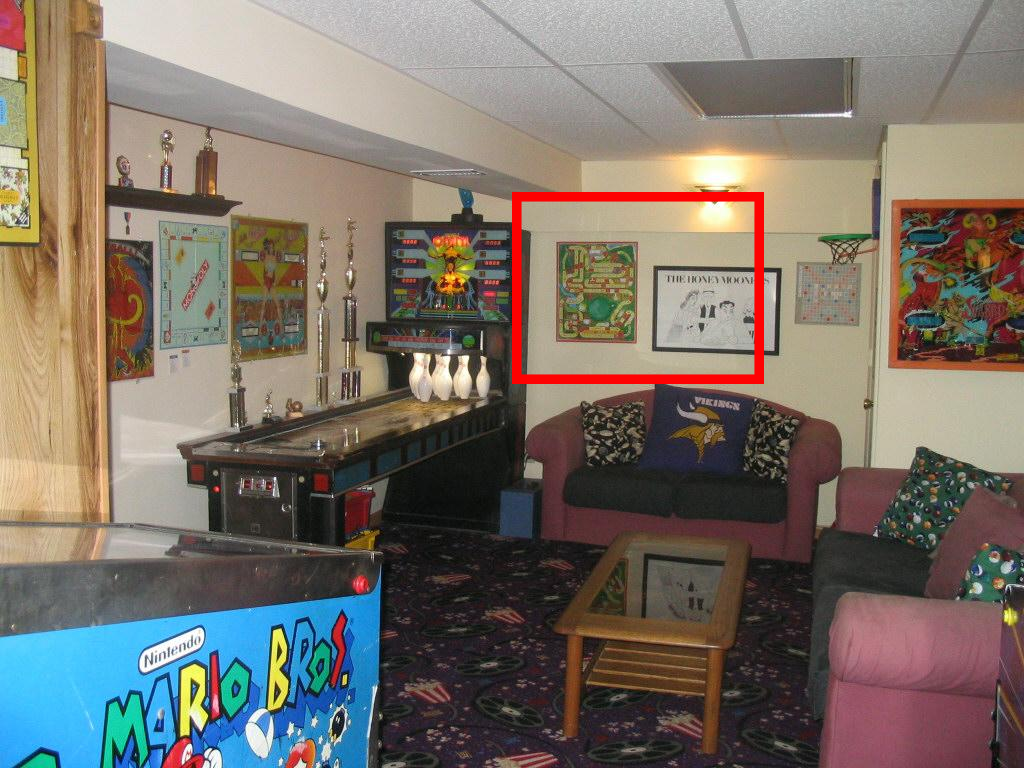
\includegraphics[height=0.20\linewidth]{article2/images/tele1.png}\\ 
  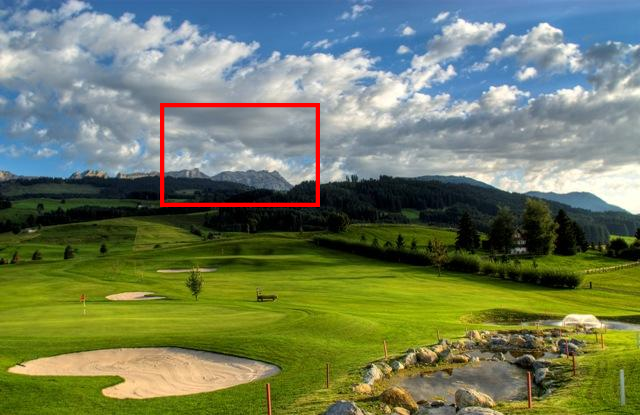
\includegraphics[height=0.20\linewidth]{article2/images/cloud2.png}&
  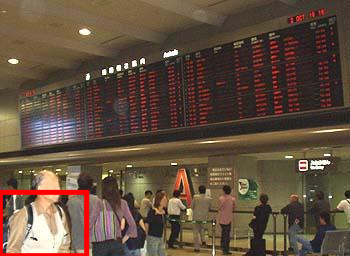
\includegraphics[height=0.20\linewidth]{article2/images/man2.png} &
  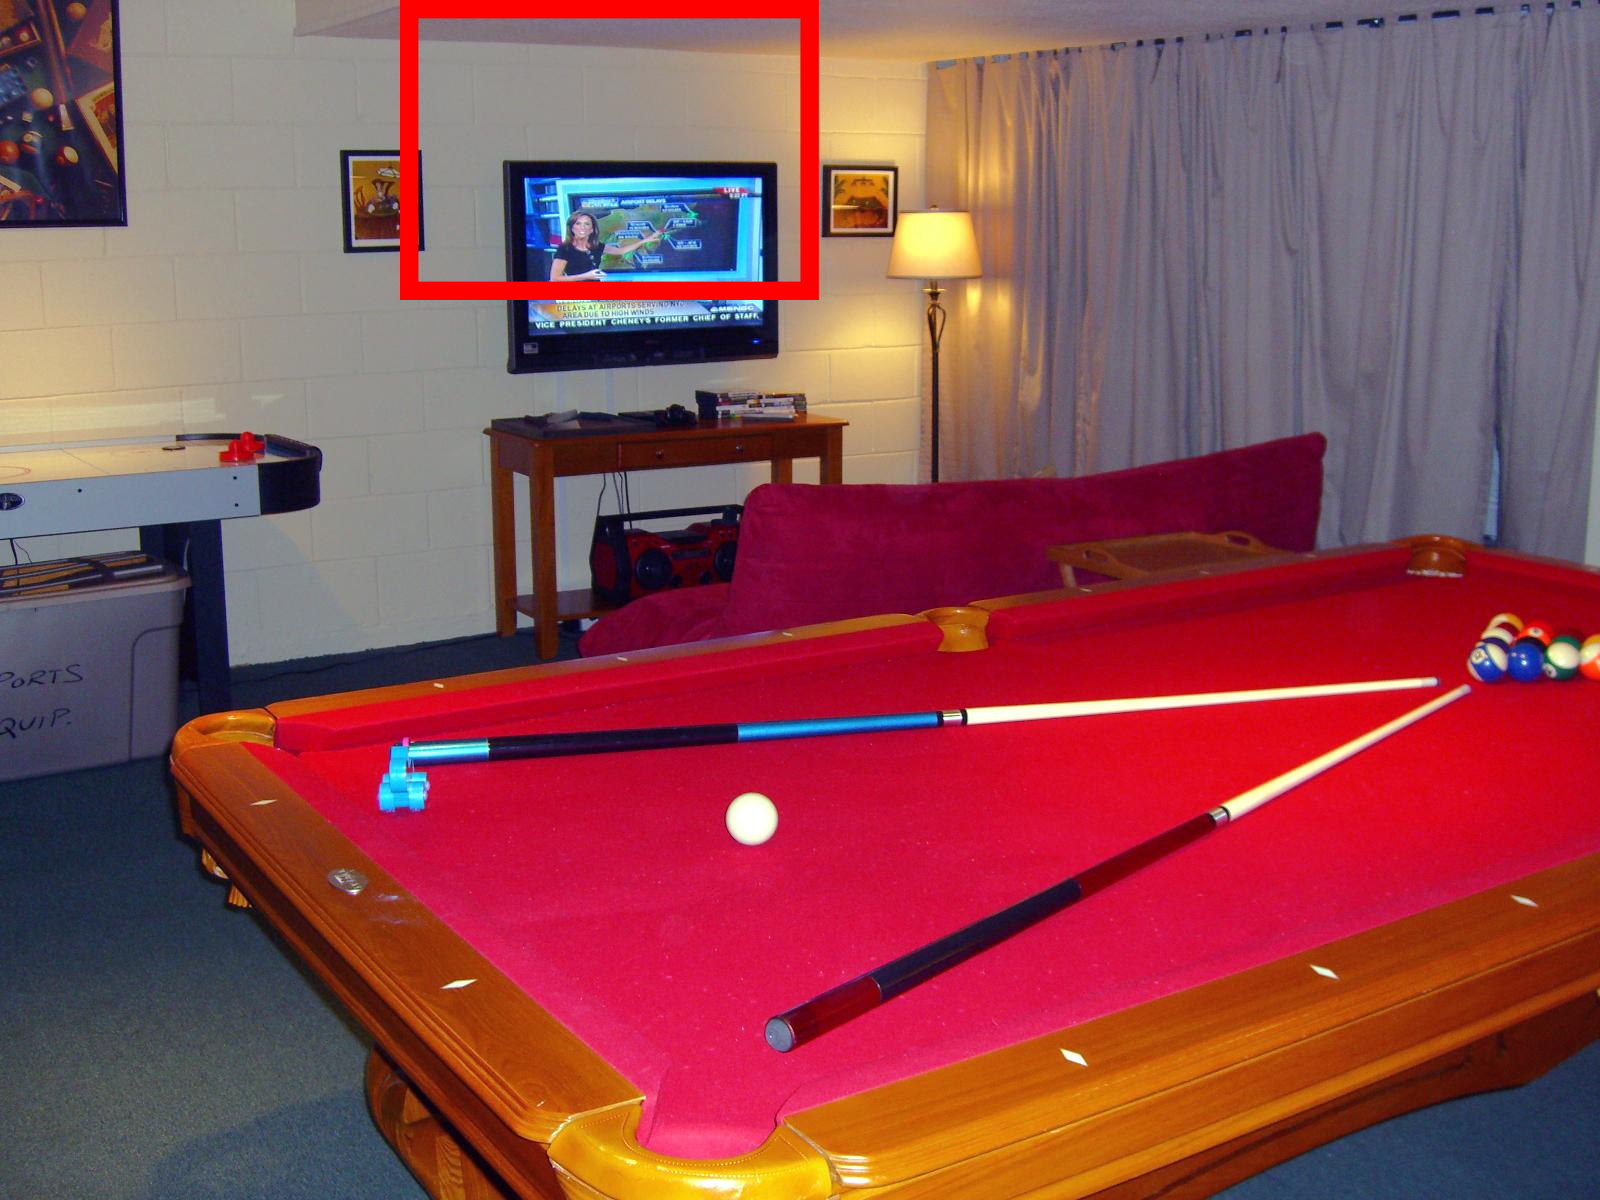
\includegraphics[height=0.20\linewidth]{article2/images/tele2.png}\\ 
\end{tabular}
\end{center}

   \caption[Scene images and OB detections]{{\it Left:} Cloud {\it Middle:} Man {\it Right:} Television. {\it
   Top:} False Detections {\it Bottom:} True Detections. Images from {\bf
   SUN}~\citep{Xiao:2010} for which we compute the OB representation and display the
   bounding box around the average position of various objects detectors. For
   instance, the \textit{television} detector can be viewed either as a
   \textit{television} detector or a \textit{rectangle} shape detector i.e.
   high-order statistical properties of the image.} \label{fig:images} 
\end{figure*}


%\begin{figure}
%\centering
%\includegraphics[height=6.2cm]{eijkel2}
%\caption{One kernel at $x_s$ (\emph{dotted kernel}) or two kernels at
%$x_i$ and $x_j$ (\textit{left and right}) lead to the same summed estimate
%at $x_s$. This shows a figure consisting of different types of
%lines. Elements of the figure described in the caption should be set in
%italics, in parentheses, as shown in this sample caption.}
%\label{fig:example}
%\end{figure}


\section{Scene Categorization with Object-Bank} \label{sec:ob}

Let us begin by introducing the approach of the OB
project \citep{LiJiaLi10}.
%
First, the $177$ most useful (or frequent) objects were selected from
popular image datasets such as LabelMe \citep{labelme}, ImageNet
\citep{imagenet} and Flickr.
%
For each of these $177$ objects, a specific detector, existing in the
literature \citep{Felzen08,Hoiem05}, was trained.
%
Every detector is composed of $2$ {\em root filters} depending on the
pose, each one coming with its own deformable pattern of parts, e.g., there
is one root filter for the front-view of a bike and one for the
side-view.
%
These $354=177\times 2$ part-based filters (each composed by a root and its parts)
are used to produce features of natural images.
%
For a given image, a filter is convolved at $6$ different scales. At
each scale, the max-response among $21=1+4+16$ positions (whole image,
quadrants, quadrants within each quadrant) is kept, producing a
response map of dimension $126=6\times 21$.
%
All $2\times 177$ maps are finally concatenated to produce an over-complete
representation $x\in\mathbb{R}^{44,604}$ of the original image.
%

In the original OB paper \citep{LiJiaLi10}, classifiers for scene
categorization are learned directly on these feature vectors of
dimension $44,604$.
%
More precisely, $C$ classifiers (Linear SVM or
Logistic Regression) are trained in a $1$-versus-all setting in order to predict the
correct scene category $y_{\textrm{category}}(x)$ among $C$ different
categories.
%
Various strategies using structured sparsity with combinations
  of $\ell_1/\ell_2$ norms have been proposed to handle the
  very large input.

\section{Unsupervised Feature Learning}\label{sec:feat}

% motivation
The approach of OB for the task of scene categorization,
based on specific object detectors, is appealing since it works well
in practice.
%
This suggests that a scene is better recognized by first identifying
basic objects and then exploiting the underlying semantics in the
dependencies between the corresponding detectors.
%

However, it appears that none of the individual object detectors
reaches a recognition precision of more than $30\%$. Hence, one may
question whether the ideal view that inspired this approach (and
expressed above) is indeed the reason of OB's success.
%
Alternatively, one may hypothesize that the $44,604$ OB features are
more useful for scene categorization because they represent high level
statistical properties of images than because they precisely report the 
absence/presence of objects $-$ see Figure~\ref{fig:images}.
%
OB tried structured sparsity to handle this feature selection but there may be
  other ways -- simpler or not.

This paper investigates several ways of learning higher-level features
{\bf on top of} the high dimensional representation provided by OB,
expecting that capturing further structure may improve categorization
performance. Our approach employs \textit{unsupervised feature
  learning/extraction} algorithms, i.e. generic feature extraction
methods which were not developed specifically for images. We will
consider both standard Principal Component Analysis and
Contractive Auto-Encoders
\citep{Rifai+al-2011}. The latter is a recent machine
learning method which has proved to be a robust feature extraction
tool.

\subsection{Principal Component Analysis}

Principal Component Analysis (PCA)~\citep{Pearson-1901,Hotelling1933} 
is the most prevalent technique for
linear dimensionality reduction. A PCA with $k$ components finds the $k$
orthonormal directions of projection in input space that retain most of the
\textit{variance} of the training data. These correspond to the eigenvectors
associated with the leading eigenvalues of the training data's covariance
matrix. Principal components are
ordered, so that the first corresponds to the direction along which the data varies the
most (largest eigenvalue), etc\ldots 

Since we will consider an auto-encoder variant (presented next),
% as an alternative feature extractor to PCA
we should mention here a well-known result: a linear auto-encoder with $k$
hidden units, trained to minimize squared reconstruction error, will learn
projection directions that span the same \textit{subspace} as a $k$ component
PCA~\citep{Baldi89}.  However the regularized non-linear auto-encoder variant
that we consider below is capable of extracting qualitatively different, and
usually more useful, nonlinear features.

\subsection{Contractive Auto-Encoders}

Contractive Auto-Encoders (CAEs) \citep{Rifai+al-2011} are among
the latest developments in a line of machine learning research on nonlinear
feature learning methods, that started with the success of Restricted Boltzmann
Machines~\citep{Hinton06} for pre-training deep networks, and was followed by
other variants of auto-encoders such as
sparse~\citep{ranzato-07-small,Koray-08,Goodfellow2009} and  denoising
auto-encoders~\citep{VincentPLarochelleH2008}.
%,Vincent-JMLR-2010}.  
It was selected here mainly due to its practical ease of use and recent
empirical successes.

Unlike PCA that decomposes the input space into leading {\em global} directions
of variations, the CAE learns features that capture local directions of
variation (in some regions of input space). This is achieved by penalizing the
norm of the Jacobian of a latent representation $h(x)$ with respect to its
input $x$ at training samples. Rifai et al.~\citep{Rifai+al-2011} show that the
resulting features provide a local coordinate system for a low dimensional
manifold of the input space. This corresponds to an atlas of charts, each
corresponding to a different region in input space, associated with a different
set of active latent features. One can think about this as being similar to a
mixture of PCAs, each computed on a different set of training samples that were
grouped together using a similarity criterion (and corresponding to a different
input region), but without using an independent parametrization for each
component of the mixture, i.e., allowing to generalize across the charts, and
away from the training examples.

In the following, we summarize the formulation of the CAE as a regularized
extension of a basic Auto-Encoder (AE). In our experiments, the parametrization
of this AE consists in a non-linear encoder or latent representation $h$ of $m$
hidden units with a linear decoder or reconstruction $g$ towards an input space
of dimension $d$.\\

 Formally, the latent variables
are parametrized by:
\begin{equation}
\label{eq:AE-encoder}
h(x) = s(W x+b_h),
\end{equation}
where $s$ is the element-wise logistic sigmoid
$s(z)=\frac{1}{1+e^{-z}}$, $W\in\mathcal{M}_{m\times d}(\mathbb{R})$ and $b_h\in\mathbb{R}^{m}$ are the parameters to be
learned during training.  Conversely, the units of the decoder are linear
projections of $h(x)$ back into the input space:
\begin{equation}
\label{eq:AE-decoder}
g(h(x)) = W^Th(x).
\end{equation}
Using mean squared error as the reconstruction objective and the
L$2$-norm of the Jacobian of $h$ with respect to $x$ as
regularization, training is carried out by minimizing the following
criterion by stochastic gradient descent:
\begin{eqnarray}
\label{eq:CAE-objective}
\mathcal{J}_{\mathrm{CAE}}(\Theta) = \sum_{x \in {\cal D}} \|x - g(h(x))\|^2 +
\lambda \sum_{i=1}^{m}\sum_{j=1}^{d}\left|\frac{\partial h_{i}}{\partial x_{j}}(x)\right|^2 ,
\end{eqnarray}

where $\Theta=\{ W,b_{h}\}$, ${\cal D}=\{x^{(i)}\}_{i=1,\dots,n}$ corresponds
to a set of $n$ training samples $x\in\mathbb{R}^{d}$ and $\lambda$ is a hyper-parameter
controlling the level of contraction of $h$.
%
A notable difference between CAEs and PCA is that features extracted by CAEs
are non-linear w.r.t. the inputs, so that multiple layers of CAEs can be
usefully composed (stacked), whereas stacking linear PCAs is pointless.

\section{Extracting Better Features with Advanced Combination
  Strategies} \label{sec:combi} %\ref{sec:pwork}


In this work, we study two different sub-structures of OB. We consider
the \textit{pose} response defined by the output of only one part-based filter at all
positions and scales, and the \textit{object} response which is the concatenation of all
\textit{pose} responses associated to an object. Combination
strategies are depicted in Figure~\ref{fig:architectures}.

\subsection{Simplistic Strategies: Mean and Max Pooling}

The idea of pooling responses at different locations
or poses has been successfully used in
Convolutional Neural Networks such as LeNet-$5$
\citep{Lecun99objectrecognition} and other visual processing \citep{Serre05}
architectures inspired by the visual cortex.

Here, we pool the $252$ responses of each object detector into one component
(using the mean or max operator) leading to a representation of size
$177=44604/252$. It corresponds to the mean/max over the object responses at
different scales and locations. One may view the object max responses as
features encoding absence/presence of objects while discarding all the
information about the detector's positions. 



\begin{figure*}
\begin{center}
\begin{tabular}{cccc}
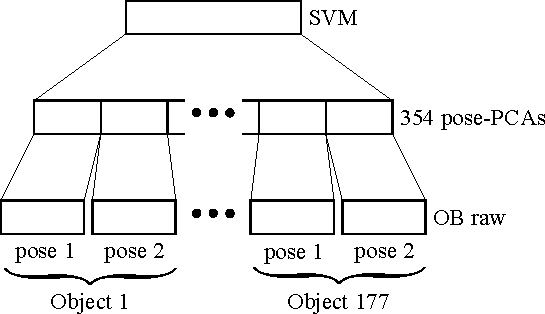
\includegraphics[width=0.33\linewidth]
{article2/images/PosePCAs.pdf}&
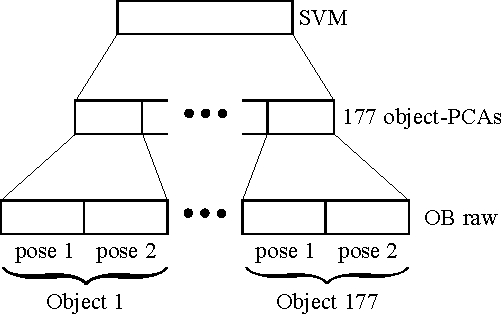
\includegraphics[width=0.33\linewidth]
{article2/images/ObjectPCAs.pdf}&
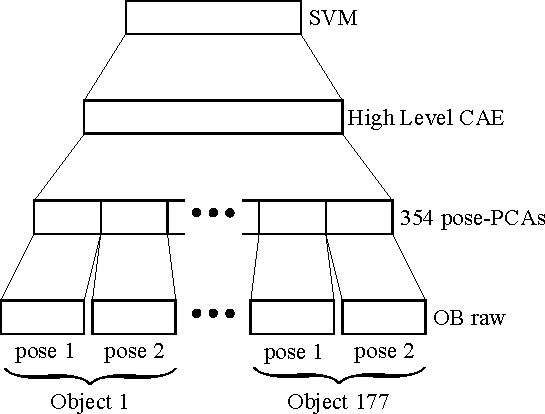
\includegraphics[width=0.33\linewidth]
{article2/images/HighLevelCAE.pdf}\\
\end{tabular}
\end{center}

\caption[Different Combination Strategies]{{\bf Different Combination Strategies} (a) and (b) \textit{pose} and
\textit{object} PCAs (c) high-level CAE: \textit{pose}-PCA as dimensionality
reduction technique in the first layer and a CAE stacked on top. We denote it
high-level because it can learn \textit{context information} i.e. plausible
joint appearance of different objects.}

\label{fig:architectures}
\end{figure*}

\subsection{Combination Strategies with PCA}

PCA is a standard method for extracting features from high dimensional input, so 
it is a good starting point. However, as we find in our experiments, exploiting
the particular structure of the data, e.g., according to poses, scales, and
locations, can yield to improved results.

\vspace{-0.2cm}
\paragraph{Whole PCA.}
An ordinary PCA is trained on the raw output of OB ($x \in\mathbb{R}^{44,604}$)
without looking for any structure.  Given the high-dimensionality of OB's
representation, we used the Randomized PCA algorithm of the
scikits toolbox\footnote{Available from \textit{http://scikits.appspot.com/}}.


\vspace{-0.2cm} \paragraph{Pose-PCA.} Each of the two \textit{poses} associated
with each \textit{object} detector is considered independently.  This results
in $354=2\times 177$ different PCAs, which  are trained on \textit{pose}
outputs ($x\in\mathbb{R}^{126}$) -- see Figure~\ref{fig:architectures}. 

\vspace{-0.2cm}
\paragraph{Object-PCA.}
Only each \textit{object} response ($x \in\mathbb{R}^{252}$) is considered
separately, therefore $177$ PCAs are trained in total.  It allows the model to
capture variations among all \textit{pose} responses at various scales and
positions -- see Figure~\ref{fig:architectures}.\\ 


Note that, in all cases,  whitening the PCA (i.e. dividing each eigenvector's
response by the corresponding squared root eigenvalue) performs very poorly.
For post-processing, the PCA outputs $\tilde{x}$ are always normalized:
$\tilde{x}\leftarrow (\tilde{x}-\mu)/\sigma $ according to mean $\mu$ and the
deviation $\sigma$ of the whole, per \textit{object} or per \textit{pose} PCA
outputs. Thereby, we ensure contributions from all \textit{objects} or
\textit{poses} to be in the same range.  The number of components in all cases
has been selected according to the classification accuracy estimated by
$5$-fold cross-validation.


\subsection{Improving upon PCA with CAE}

% interesting to capture patterns of variation for one object detector among various scales and size
% 1) variations intra-pose 2) variations among poses,scale and position


% % image -> Hog -> scale (6 scales differents) -> convol (x 2 poses: face et cote) 
% % max pool sur tt image, dans 4 cardants et 16 cadrants. -> 21 positions de
% % candidats max pour 1 scale.

% interesting to capture patterns of variation for one object detector among various scales and size
% 1) variations intra-pose 2) variations among poses,scale and position

% 44604 currently CAE not scaling up to this dim.
% take advantage of struct. (output of 177 obj detectors at different
% poses, scales and positions)

% % 1ere couche:

% % Pour chaque type d'objet/pose, on carcterise les invariances
% % posititon/scale.
% % CAE entraine pour chacune des 177x2 poses sur input 21pos*6scales vers dim 100.
% % (+SVM)

Due to hardware limitations and high-dimensional input, we could not train a
CAE on the whole OB output (``whole CAE''). However, we address this problem 
with the sequential feature extraction steps below.

%\paragraph{High- CAE.}
\label{sec:highlevel}
To overcome the tractability problem that forbids a CAE to be
trained on the whole OB output, we preprocess it by using the
\textit{pose}-PCAs as a dimensionality reduction method. We keep
only the $5$ first components of each \textit{pose}. Given this
low-dimensional representation (of dimension $1,770$), we are able to
train a CAE -- see Figure~\ref{fig:architectures}.
%
The CAE has a global view of all object detectors and
can thus learn to capture {\em context information}, defined by the
joint appearance of combinations of various objects. Moreover, instead
of using an SVM on top of the learned representations, we can use a
Multi-Layer Perceptron whose weights would be initialized by those of
this CAE. This setting is where the CAE has shown to perform
best in practice \citep{Salah+al-2011}.

\section{Experiments} \label{sec:exp}


\subsection{Datasets}


We evaluate our approach on $3$ scene datasets, cluttered indoor images (MIT
Indoor Scene),  natural scenes ($15$-Scenes), and event/activity images
(UIUC-Sports). Images from a large scale scene recognition dataset (SUN-$397$
database) have also been used for unsupervised learning. 
%\vspace{-1ex}
\begin{itemize}
  \item {\bf{MIT Indoor}} is composed of $67$ categories and, following
\citep{LiJiaLi10,Quattoni09}, we used $80$ images from each category for
training and $20$ for testing.

\item {\bf{15-Scenes}} is a dataset of $15$ natural scene
classes. According to \citep{Lazebnik06}, we used $100$ images per class for
training and the rest for testing. 

\item {\bf{UIUC-Sports}} contains $8$ event classes.  We
randomly chose $70$ / $60$ images for our training / test set respectively,
following the setting of \citep{LiJiaLi10,LiJiaLi07}.

\item {\bf{SUN-397}} contains a full variety of $397$  well sampled
scene categories ($100$ samples per class) composed of $108,754$ images in total.
\end{itemize}





\subsection{Tasks}
\label{sec:results}

We consider $3$ different tasks to evaluate and compare the considered
combination strategies. In particular, various supervision settings
for learning the CAE are explored. Indeed, a great advantage of this
kind of method is that it can make use of vast quantities of unlabeled
examples to improve its representations. We thus illustrate this by
proposing experiments in which the CAE has been trained in supervised or
in semi-supervised way and also in a transfer context.

\paragraph{MIT Indoor (plain).} 

Only the official training set of the MIT Indoor scene dataset
($5,360$ images) is used for unsupervised feature learning.
%
Each representation is evaluated by training a linear SVM on top of
the learned features.

\begin{table*}
\begin{center}
\begin{tabular}{l|c|c}
            & MIT               & MIT+SUN \\
            & {\it (plain)}     & {\it (semi-supervised)}   \\
\hline
\textit{object}-MAX + SVM   & $24.3\%$  & --   \\  
\textit{object}-MEAN + SVM  & $41.0\%$  & -- \\  
\hline
\textit{whole}-PCA + SVM  & $40.2\%$  & --            \\  
\textit{object}-PCA + SVM & $42.6\%$ & $46.1\%$   \\  
\textit{pose}-PCA  + SVM  & $40.1\%$ & $46.0\%$  \\  
\hline
\textit{pose}-PCA  + MLP  & $42.9\%$ & $46.3\%$  \\  
\textit{pose}-PCA + CAE (MLP) & $\mathbf{44.0\%}$  & $\mathbf{49.1\%}$\\
\hline
\hline
Object Bank + SVM & $37.6\%$  &  -- \\
Object Bank + rbf-SVM & $37.7\%$  & --\\ 
\hline
DPM + Gist + SP & $43.1\%$ & --   \\  
\hline
\hline
Improvement w.r.t. Object Bank & $+6.4\%$ & $+11.5\%$ \\ 
\hline
\end{tabular}
\end{center}

\caption[MIT Indoor Performance]{\label{tab:res1} {\bf MIT Indoor.} Results are reported on the
official split \citep{Quattoni09} for all combination strategies described in
Section~\ref{sec:combi}.  Only the unsupervised feature learning strategies
(PCA and CAE based) \textit{can} benefit from the addition of unlabeled scenes
from SUN. Object Bank + SVM refers to the original system~\citep{LiJiaLi10} and DPM +
Gist + SP~\citep{Pandey11} corresponds to the state-of-the-art method on MIT Indoor.  } 

\end{table*}


\paragraph{MIT+SUN (semi-supervised).} This task, like the previous one, uses
the official train/test split of the MIT Indoor scene dataset for its
supervised training and evaluation of scene categorization performance. For the
initial unsupervised feature extraction however, we augmented the MIT Indoor
training set with the whole dataset of images from SUN-397 ($108,754$ images).
This yields a total of $123,034$ images for unsupervised feature learning and
corresponds to a \textit{semi-supervised} setting.
%
Our motivation for adding scene images from SUN, besides increasing the number
of training samples, is that on MIT Indoor, which contains only indoor scenes,
OB detectors specialized on outdoor objects would likely be mostly inactive (as
a sailboat detector applied on indoor scenes) and irrelevant, introducing an
harmful noise in the unsupervised feature learning.  As SUN is composed of a
wide range of indoor and outdoor scene images, its addition to MIT Indoor
ensures that each detector meaningfully covers its whole range of activity
(having a "balanced" number of positives/negatives detections through the
training set) and the feature extraction methods can be efficiently trained to
capture it.
%

One may object that training on additional images does not provide a fair
comparison w.r.t. the original OB method. Nevertheless, we recall that (1)
the supervised classifiers do not benefit from these additional examples and
(2) object detectors which are the core of OB representations (and all
detector-based approaches) have also obviously been trained on
\textit{additional} images.


\paragraph{UIUC-Sports and 15-Scenes (transfer).} We would also like to
evaluate the discriminative power of the various representations learned on the
MIT+SUN dataset, but on new scene images and categories that were \textit{not}
part of the MIT+SUN dataset.  This might be useful in case other researchers
would like to use our compact representation on a different set of images.
%in the same way they use low-level feature detectors
 Using the representation output by the feature extractors learned with
 MIT+SUN, we train and evaluate classifiers for scene categorization on images
 from UIUC-Sports and 15-Scenes (not used during unsupervised training). This
 corresponds to a \textit{transfer learning} setting for the feature
 extractors.
%
\begin{table*}
\begin{center}
\begin{tabular}{l|c|c}
          & UIUC-Sports     &  $15$-SCENES \\
%LScSPM \citep{Gao10} & $\mathbf{85.30\%}$  & $\mathbf{89.70\%}$ \\  
\hline
\textit{object}-MAX  + SVM   & \mbox{~~~~}$67.23\pm1.29\%$\mbox{~~~~}  & \mbox{~~~~}$71.08\pm0.57\%$\mbox{~~~~}  \\  % hack moche pour donner un peu d'air au tableau
\textit{object}-MEAN + SVM   & $81.88\pm1.16\%$ & $83.17\pm0.53\%$  \\  
\hline
\textit{object}-PCA + SVM  & $83.90\pm1.67\%$        & $85.58\pm0.48\%$  \\  
\textit{pose}-PCA + SVM    & $83.81\pm2.22\%$        & $85.69\pm0.39\%$  \\  
\hline
\textit{pose}-PCA + MLP    & $84.29\pm2.23\%$        &  $84.93\pm0.39\%$  \\  
\textit{pose}-PCA + CAE (MLP) & $\mathbf{85.13\pm1.07\%}$     &  $\mathbf{86.44\pm0.21\%}$ \\
\hline
\hline
Object Bank + SVM   & $78.90\%$  & $80.98\%$ \\  
Object Bank + rbf-SVM & $78.56\pm1.50\%$ & $83.71\pm0.64\%$ \\
\hline
Improvement w.r.t. OB & $+6.23\%$ & $+5.46\%$ \\
\hline
\end{tabular}
\end{center}

\caption[Transfer Performances on UIUC-Sports and 15-SCENES]{\label{tab:res2} {\bf UIUC Sports and 15-Scenes} Results are reported
for $10$ random splits (available at www.anonymous.org) and compared to the
    original OB results~\citep{LiJiaLi10} - Object Bank + SVM - on one single
    split.}

\end{table*}

\subsection{SVMs on Features Learned with each Strategy} 

In order to evaluate the quality of the features generated by each
strategy, a linear SVM is trained on the features extracted 
by each combination method.
%
We used LibLinear \citep{liblinear} as SVM solver and chose the best C
according to $5$-fold cross-validation scheme.
%
We compare accuracies obtained by features provided by all considered
combination methods against the original OB performances~\citep{LiJiaLi10}. 
%state-of-the-art results
%from~\citep{LiJiaLi10,Gao10,Pandey11}.
% on several datasets described below.
%
Results obtained with SVM classifiers on all MIT-related tasks are
displayed in Table~\ref{tab:res1} and those concerning UIUC and
15-scenes in Table~\ref{tab:res2}.

%
The simplistic strategy \textit{object} mean-pooling performs surprisingly well
on all datasets and tasks whereas \textit{object} max-pooling obtained the
worst results.  It suggests that taking the mean response of an object detector
across various scales and positions is actually meaningful compared to consider
presence/absence of objects as max-pooling does.
%
%CAEs have not been trained on plain MIT because the number of training images
%was too small to achieve interesting performances without fine-tuning (see
%next section), but a careful use of PCA is already beneficial.
%

On MIT and MIT+SUN, \textit{object} or \textit{pose} PCAs reach almost the same
range of performance slightly above the current state-of-the-art performances
\citep{Pandey11}, except for whole-PCA which performs poorly: one must consider
the structure of OB to combine features efficiently. In the experiments,
keeping the $10$ (resp. $15$) first principal components gave us the best
results for pose-PCA (resp. object-PCA).

%
Besides, Table~\ref{tab:dim} shows that both PCAs and PCA+CAE allow a huge
reduction of the dimension of the OB feature representation.
%
%Nevertheless, components obtained with \textit{pose}-PCA and filters learned
%by the \textit{pose}-CAE are quite different, as depicted in
%Figure~\ref{fig:short}.

Results obtained for the UIUC-Sports and 15-Scenes transfer learning tasks are
displayed in Table~\ref{tab:res2}. Representations learned on MIT+SUN
generalize quite well and can be easily used for other datasets even if images
from those datasets  have not been seen at all during unsupervised learning.

\begin{table*}
 \begin{center}
\resizebox{1\linewidth}{!}{
\begin{tabular}{c|c|c|c|c|c}
Object-Bank &  Pooling & \textit{whole}-PCA & \textit{object}-PCA & \textit{pose}-PCA & \textit{pose}-PCA+CAE \\
\hline
$44,604$ & $177$ & $1,300$ & $2,655$ & $1,770$ & $1,000$ \\
\end{tabular}
}
\end{center}
\caption[Dimensionality Reduction]{\label{tab:dim} {\bf Dimensionality Reduction.}
  Dimension of representations obtained on MIT Indoor. The \textit{pose}-PCA+CAE 
produces a compact and powerful combination.
} 
\end{table*}


\subsection{Deep Learning with Fine Tuning} Previous
work~\citep{Larochelle-jmlr-2009} on Deep Learning generally showed that the
features learned through unsupervised learning could be improved upon by
fine-tuning them through a supervised training stage. In this stage (which
follows the unsupervised pre-training stage), the features and the classifier
on top of them are together considered to be a supervised neural network, a
Multi-Layer Perception (MLP) whose hidden layer is the output of the trained
features. 
%
Hence we apply this strategy to the {\it pose} PCA+CAE architecture, keeping
the PCA transformation fixed but fine-tuning the CAE and the MLP altogether.
These results are given at the bottom of tables~\ref{tab:res1}
and~\ref{tab:res2}. The MLP are trained with early stopping on a validation set
(taken from the original training set) for $50$ epochs.

\vspace{0.1cm}

This yields $44.0\%$ test accuracy on plain MIT and
$49.1\%$ on MIT+SUN: this allows to obtain state-of-the-art performance,
with or without semi-supervised training of the CAEs, even if these
additional examples are highly beneficial.
%, {\bf 6\% above the previous state-of-the-art}~\citep{Pandey11}.
As a check, we also evaluate the effect of the unsupervised
pre-training stage by completely skipping it and only training a
regular supervised MLP of $1000$ hidden units on top of the PCA output, yielding a worse test
accuracy of $42.9\%$ on MIT and $46.3\%$ on MIT+SUN.
%
This improvement with fine-tuning on labeled data is a great advantage
for CAE compared to PCA.
%
Fine-tuning is also beneficial on UIUC-Sports and 15-Scenes. On both datasets,
this leads to an improvement of $+6\%$ and $+5\%$ w.r.t the original system.

\vspace{0.1cm}
Finally, we trained a non-linear SVM (with rbf kernel) to verify whether this
gap in performances was simply due to the replacement of a linear classifier
(SVM) by a non-linear one (MLP) or to the detectors' outputs combination. The
poor results of the rbf-SVM (see tables~\ref{tab:res1} and~\ref{tab:res2}) suggests that the
careful combination strategies are essential to reach good performance.


\begin{table*}
\begin{center}
\begin{tabular}{|c|}
\hline
\textbf{Context Semantics learned by the CAE}\\
\hline
sailboat, rock, tree, coral, blind\\
roller coaster, building, rail, keyboard, bridge\\
sailboat, autobus, bus stop, truck, ship\\
curtain, bookshelf, door, closet, rack\\
soil, seashore, rock, mountain, duck\\
attire, horse, bride, groom, bouquet\\
bookshelf, curtain, faucet, screen, cabinet\\
desktop computer, printer, wireless, computer screen\\%, computing device\\
\hline
\end{tabular}
\end{center}

\caption[Context semantics]{\label{tab:cae} {\bf Context semantics}: Names of the detectors corresponding to
the highest weights of $8$ hidden units of the CAE. These hidden units will fire
when those objects will be detected altogether. }

\end{table*}

\subsection{Use of External Semantic Information for Re-Ranking}

WordNet's~\citep{wordnet} semantic structure provide an easy way to measure word similarities.
We assume that closely related objects detectors (according to WordNet) should
fire together and could be grouped in order to build semantically meaningful features.
E.g. by grouping the output of {\it ship}, {\it sea} and {\it sun} into a
single feature, the combination's output might be useful for classifying the
``sailing'' scene category. 

In our experiments, we used the lesk distance in WordNet to extract the
neighbors of each detector's name. Some examples are depicted in
Table~\ref{tab:lesk}. Afterwards, given the score $s(x)\in\mathbb{R}^{177}$
obtained with the mean-pooling strategy from the original OB
representation $x\in\mathbb{R}^{44,604}$, we performed the following Re-Ranking
operation:
 
\begin{equation}
\label{eq:rescore}
s^{'}_{i}(x) = \sum_{j=1}^{177}s_{j}(x)\gamma^{R(i,j)} \textrm{ for }i=1,\dots,177
\end{equation}

where $\gamma\in [0,1]$ is a decay hyper-parameter tuned on a validation set.
$R(i,j)$ corresponds to the rank of the object $j$ among the neighbors of
object $i$ according to the lesk metric ($R(i,i)=0$). Results 
%on the concatenation
%of the original score $s(x)$ and its re-ranked version $s^{'}(x)$
 are presented in Table~\ref{tab:reslesk}.  The relatively small improvement
 brought by WordNet illustrates the fact that the poor intrinsic quality of the
 object detectors prevents any use of external semantic resource to improve
 their combination.

\begin{table}
    \centering
    \begin{tabular}{l|c|c|c}
    \hline
    {\it Rank} & {\bf bus} & {\bf lion} & {\bf laptop}\\
    \hline
    1. & car & tree & baggage\\
    2. & ship & dog & desktop computer\\
    3. & truck & bird & computer\\
    4. & aircraft & horse & bed\\
    5. & train & computer & door\\
    \hline
    \end{tabular}
    \caption[WordNet Semantics]{\label{tab:lesk} {\bf WordNet semantics}: Names of the detectors
    and their top-ranked neighbors according to the lesk distance computed from
    WordNet.}
\end{table}

\begin{table}
    \centering
    \begin{tabular}{l|c}
    \hline
    object-MEAN+SVM& MIT {\it(plain)}\\
    \hline
    w/o Re-Ranking & $41.03\%$ \\
    with Re-Ranking & $41.52\%$ \\
    \hline
    \end{tabular}
    \caption[Re-Ranking ]{\label{tab:reslesk} {\bf Re-Ranking}: Results are reported on
    the official split \citep{Quattoni09}. Object-mean+SVM refers to the
    mean-pooling strategy with and w/o the Re-Ranking transformation.} 
\end{table}


% the
%first one, this leads to similar performances as the state-of-the-art,
%LScSPM~\citep{Gao10}. Note that LScSPM do not rely on detectors but use
%a more standard approach for image classification based on local
%feature descriptors.
%

\section{Discussion}\label{sec:disc}

In this work, we add one or more levels of trained representations on top of
the layer of object and part detectors (OB features) that have constituted the
basis of very promising trend of approach for scene
classification~\citep{LiJiaLi10}.
%
These higher-level representations are mostly trained in an unsupervised way,
following the trend of so-called Deep
Learning~\citep{Hinton06,Bengio-2009,Jarrett-ICCV2009}, but can be fine-tuned
using the supervised detection objective.
%

These learned representations capture statistical dependencies in the
co-occurrence of detections the object detectors from~\citep{LiJiaLi10}.  In
fact, one can see in Table~\ref{tab:cae} plausible contexts of joint appearance
of several objects learned by the CAE.
%
These detectors, which can be quite imperfect when seen as actual detectors,
contain a lot of information when combined altogether. However, the uncertainty
of detectors makes it hard to combine using external semantic sources such as
WordNet. As reported in Table~\ref{tab:reslesk}, we observe a slight
improvement ($+0.5\%$) using our Re-Ranking strategy and lesk words'
similarities.
%seen as features that can be computed at many scales and locations. 
%
The extraction of those {\it context semantics} with unsupervised
feature-learning algorithms has empirically shown better performances but these
semantics are inherent to the detectors outputs and can not be easily combined
with any known predefined semantic system such as the one defined in WordNet.

%

In particular, we find that Contractive
Auto-Encoder~\citep{Rifai+al-2011} can substantially improve
performance on top of \textit{pose} PCAs as a way to extract non-linear
dependencies between these lower-level OB detectors (especially when
fine-tuned). They also improve greatly upon the use of the detectors as inputs
to an SVM or a logistic regression (which were, with structured regularization,
the original methods used by OB).
%

This trained post-processing allows us to reach the state-of-the-art on MIT
Indoor and UIUC ($85.13\%$ against $85.30\%$ obtained by LScSPM~\citep{Gao10})
while being competitive on 15-scenes ($86.44\%$ also versus $89.70\%$ LScSPM). 
%
On these last two datasets, we reach the best performance for methods only
relying on object/part detectors. Compared to other kinds of methods, we are
limited by the accuracy of those detectors (only trained on HOG features),
whereas competitive methods can make use of other descriptors such as
SIFT~\citep{Gao10}, known to achieve excellent performance in image recognition.


Besides its good accuracies, it is worth noting that the feature representation
obtained by the {\it pose} PCA+CAE is also very compact, allowing a 97\%
reduction compared to the original data (see Table~\ref{tab:dim}).  Handling a
dense input of dimension $44,604$ is not a common thing. By providing this
compact representation, we think that researchers will be able to use the rich
information provided by OB in the same way they use low-level image descriptors
such as SIFT.
 

%\section{Future Work}\label{sec:future}

As future work, we are planning other ways of combining OB features
e.g. considering the output of all detectors at a given scale and
position and combine them afterwards in a hierarchical manner.  This
would be a kind of dual view of the OB features. Other plausible
departures could take into account the topology (e.g. spatial
structure) of the pattern of detections, rather than treat the
response at each location and scale as an attribute and the set of
attributes as unordered. This could be done in the same spirit as in
Convolutional Networks~\citep{Lecun99objectrecognition}, aggregating
the responses for various objects detectors/locations/scales in a way
that takes explicitly into account the object category, location and
scale of each response, similarly to the way filter outputs at
neighboring locations are pooled in each layer of a Convolutional
Network.

\section{Acknowledgments} We would like to thank Gloria Zen for her helpful
comments.  This work was supported by NSERC, CIFAR, the Canada Research Chairs,
Compute Canada and by the French ANR Project ASAP ANR-09-EMER-001. Codes for
the experiments have been implemented using Theano~\citep{bergstra+al:2010-scipy} Machine Learning library.

%\bibliographystyle{plain}
%{\small
%\bibliography{strings,strings-short,strings-shorter,ml,myrefs,aigaion-short}
%}




%\end{document}
